\chapter{Ulepszenia dla silnika szachowego}
\label{ch:implementacja-silnika-szachowego}

Po opisanych w rozdziale drugim krokach silnik stał się zdolny do samodzielnej gry.
W poniższej części opisane zostały zagadnienia związane z poprawą szybkości i precyzji działania systemu.
W pierwszej kolejności skupiono się na ulepszeniu przeszukiwania ruchów w celu znalezienia najlepszego z posunięć.
Następnie opisano zmiany heurystyki planszy pozwalające silnikowi na~lepszą ocenę bieżącej sytuacji gry.

\section{Ulepszenia dla wyszukiwania}
\label{sec:ulepszenia-dla-wyszukiwania}


\subsection{Biblioteka otwarć}
\label{subsec:biblioteka-otwarc}

\subsubsection{Opis zagadnienia}
Głównym problemem, który należało rozwiązać, były otwarcia partii rozgrywanych przez silnik.
Gry szachowe zawsze rozpoczynają się z tego samego położenia, więc wiadomo, że~system znajdzie się w wielu pozycjach bezpośrednio wynikających z pierwszych posunięć.
Program natomiast poświęcał na obliczenia wiele czasu, który lepiej byłoby spożytkować w~środkowym etapie rozgrywki.

Profesjonalni gracze, korzystając z dorobku i doświadczenia wielu pokoleń szachistów, zapamiętują pierwsze posunięcia do wykonania.
Tym samym oszczędzają czas, który pozostaje na bardziej złożone pozycje w środkowej fazie gry.

\subsubsection{Implementacja}
W celu zaimplementowania biblioteki otwarć, dostępne posunięcia czytane są z pliku, a~następnie zapisywane przy inicjalizacji silnika do HashMapy \texttt{<String, []Moves>}.
Podczas działania silnika, FEN aktualnej pozycji porównywalny jest z dostępnymi kluczami, a ruch losowo wybierany spośród dostępnych w tablicy.
W przypadku nieznalezienia klucza program przechodzi do gry środkowej z wykorzystaniem algorytmu negaMax.

W literaturze znanych jest wiele formatów zapisu biblioteki otwarć, np.\ EPD, PGN czy~Bin-format.
System wykorzystuje bibliotekę wygenerowaną przez Sebastiana Lague i~dostępną na licencji MIT w~implementacji jego silnika~\cite*{opening-library}.
\subsubsection{Rezultat}
Efektem prac stał się silnik, który początkowe posunięcia wykonuje za pomocą podpiętej biblioteki otwarć.
Dzięki temu pierwsze ruchy wykonywane są bardzo szybko, pozostawiając cenny czas obliczeniowy na dalszą grę, tym samym zwiększając precyzję.

We wcześniejszej wersji silnik był deterministyczny, to jest, dla konkretnej głębokości i pozycji, algorytm zwracał ten sam najlepszy ruch.
Dodatkowym atutem stała się jego nieprzewidywalność.
Początkowe posunięcia są zrandomizowane, co pozwala na jego testowanie w większej ilości wariantów, a także umila rozgrywkę użytkownikowi.

\subsection{Alfa-Beta cięcie}
\label{subsec:alfa-beta-ciecie}
\subsubsection{Opis zagadnienia}
Poprawne wykonanie algorytmu negaMax nie gwarantuje jego skuteczności.
Wraz z~pogłębianiem wyszukiwania rośnie również liczba wierzchołków, które należy odwiedzić.
Uśredniając, liczba dzieci, to jest pozycji wynikających z wykonania ruchu, dla danego rodzica w szachach wynosi $35$. \cite*{branching-factor}
Własność ta nazywa się współczynnikiem rozgałęzienia (ang.~\textit{branching~factor}).

Do minimalizacji liczby odwiedzonych węzłów wykorzystuje się alfa-beta cięcia.
Jest to przykład algorytmu metody podziału i ograniczeń, a jego skuteczność w dużym stopniu zależy~od kolejności przeszukiwanych ruchów.
Zakładając ułożenie posunięć od najlepszego, algorytm wykona najwięcej cięć, co w efekcie skutkować będzie zmniejszeniem liczby odwiedzonych wierzchołków dla głębokości według wzoru z tabeli:

\begin{table}[htb] \small
\centering
\caption{Teoretyczny limit alfa-beta cięcia dla współczynnika rozgałęzienia $b_f = 35$}
\label{tab:alfa-beat}
\renewcommand{\arraystretch}{1.5}
\begin{tabular}{|c|c|c|}\hline
Głębokość $n$ & ${b_{f}}^{n}$ & $b_{f}^{\lceil \frac{n}{2} \rceil} + b_{f}^{\lfloor \frac{n}{2} \rfloor} - 1$\\ \hline\hline

$1$ & $35$ & $35$\\ \hline
$2$ & $1225$ & $69$\\ \hline
$3$ & $42 875$ & $1259$\\ \hline
$\vdots$ & $\vdots$ & $\vdots$\\ \hline
$10$ & $2,76 * 10^{15}$ & $1,05 * 10^{8}$\\ \hline

\end{tabular}
\end{table}

Posortowanie ruchów od najgorszych, spowoduje brak możliwych cięć, a tym samym wynik będzie identyczny, jak przy algorytmie bez implementacji alfa-beta cięcia.


\subsubsection{Implementacja}

Algorytm alfa-beta cięcia jest edycją kodu funkcji negaMax \ref{lst:drugi}.
$\alpha$ oraz $\beta$ zostają dodane jako argumenty.
W sytuacji, gdy \texttt{score} $>$ \texttt{bestMoveValue} oraz $\alpha >$ \texttt{bestMoveValue}, $\alpha$~zostaje zaktualizowana na \texttt{bestMoveValue}.
Jeśli \texttt{score} $>=\beta$ następuje odcięcie i zwracana jest wartość \texttt{bestMoveValue}.
W wywołaniach funkcji na większej głębokości $\alpha = -\beta$ oraz $\beta = -\alpha$.

\subsubsection{Rezultat}

Implementacja powyższego rozwiązania pozwoliła na zmniejszenie liczby odwiedzonych wierzchołków podczas przeszukiwania, a tym samym pozwoliła iteratywnemu pogłębianiu na~osiągnięcie lepszych rezultatów.
Realna wartość tego ulepszenia jest różna w zależności od~aktualnej pozycji na szachownicy.
\subsection{Ewaluacja stanów cichych}
\label{subsec:ewaluacja-cichych-stanow}

\subsubsection{Opis zagadnienia}
Silnik znacznie przyspieszył znajdowanie ruchów dla danej głębokości.
Zdarzały się jednak sytuacje, że zwracane wyniki znacznie odbiegały od optymalnych.
Dla przykładu mogła zdarzyć się sytuacja, że liściem w drzewie było bicie hetmanem skoczka \cite*{duch}.
Silnik zwracał wynik heurystyki jako bardzo wysoki i wykonywał powyższy ruch.
Program nie brał jednak pod uwagę faktu, że~na~głębokości o jednej większej, hetman ten mógłby zostać zbity przez wrogiego pionka.

Taką sytuację nazywa się efektem horyzontu.
Rozwiązaniem wykonywania nieoptymalnych ruchów, było wykonanie dodatkowego wyszukiwania po osiągnięciu głębokości końcowej.
Z liścia drzewa, które poprzednio zostało oceniane heurystycznie, wyprowadzono kolejne wyszukiwanie, w którym generowane ruchy są tylko biciami.
Pozwoliło to na ocenę tak zwanych stanów cichych, czyli pozycji, gdzie nie ma żadnego dostępnego ruchu, który prowadziłby do~bicia.

\subsubsection{Implementacja}

Algorytm rozwiązujący efekt horyzontu w literaturze nosi nazwę Quiescence Search.

\begin{lstlisting}[
    language=Java,
    style=JavaStyle,
    caption=Implementacja algorytmu Quiescence Search,
    label=lst:trzeci]
    public search(depth, alpha, beta) {
        standPat = evaluator.evaluate();
        if (depth == 0) return standPat;

        if (standPat >= beta) return beta;
        if (alpha < standPat) alpha = standPat;

        moves = generator.generateCaptureMoves();
        for(Move move : moves) {
            board.makeMove(move);
            score = -search(depth-1, -beta, -alpha);
            board.unmakeMove();

            if(score >= beta) return beta;
            if(score > alpha) alpha = score;
        }
        return alpha;
    }
\end{lstlisting}

Niektóre wersje tego algorytmu, oprócz ruchów prowadzących do bicia, korzystają także z~roszad, czy~podwójnych ruchów piona, z uwagi na ich szczególny charakter.

\subsubsection{Rezultat}

W efekcie implementacji algorytmu osiągnięto silnik, który jest odporny na efekt horyzontu.
Z reguły, dodatkowe wyszukiwanie prowadzi do odwiedzenia większej liczby węzłów niż~w~przypadku zwykłego wyszukiwania.
Co warte zaznaczenia, w niektórych przypadkach, chociażby wskazanych w dodatku \ref{ch:wyniki-perft}, algorytm Quiescence Search w połączeniu z~alfa beta cięciem skutkował zmniejszeniem liczby odwiedzonych węzłów.
Ostatecznie, czy~korzystniejszym jest wyszukiwanie dla większych głębokości, czy korzystanie wyłącznie ze~stanów cichych, zależy od konkretnej sytuacji na planszy.
%\subsection{Statyczne sortowanie ruchów}
\label{subsec:sortowanie-ruchow}

\subsubsection{Opis zagadnienia}
W czasie testów zauważono, że podczas przeszukiwania drzewa nie następuje taka ilość alfa-beta cięć, która pozwalałaby na znaczne przyspieszenie obliczeń.
Rozpoczynanie przeszukiwania węzłów gry od najlepszych posunięć pozwoliłoby na osiągnięcie teoretycznego limitu wskazanego w tabeli \ref{tab:alfa-beat-limit}.
W żaden sposób nie ma jednak możliwości wskazania, który z~dostępnych ruchów prowadzi do najlepszej pozycji, przed wykonaniem tych ruchów.
Istnieją jednak posunięcia, które można rozważyć w pierwszej kolejności, ze względu na ich szczególny charakter, a~tym~samym przyspieszyć cięcie.
Jeśli sortowanie jest niezależne od wcześniejszych obliczeń, to~jest to sortowanie statyczne.

\subsubsection{Implementacja}
Sortowanie wykonano dzięki implementacji interfejsu \texttt{Comparator} w klasie \texttt{Move}.
W celu porównania pomiędzy sobą dwóch dowolnych ruchów wykorzystano następujące założenia:
\begin{itemize}
    \item Ruch, który umożliwia bicie, jest prawdopodobnie lepszy od ruchów, które nie umożliwiają bicia.
    \item Wszystkie ruchy specjalne, takie jak roszady, podwójne ruchy pionem czy promocje, są lepsze od ruchów zwykłych.
    \item Promocje do wieży i gońca należy rozważyć na końcu, gdyż są mniej wartościowe od promocji do hetmana, jednocześnie dając dostęp do tych samych ruchów.
    \item Zastosowano technikę Najbardziej wartościowa ofiara – Najmniej wartościowa atakujący (ang.~\emph{Most Valuable Victim – Least Valuable Attacker}, w~skrócie MVV-LVA). Sortuje ona~bicia zakładając, że korzystniejsze są posunięcia, w których różnica pomiędzy wartością reprezentowaną przez bierkę bijącą a bierką zbitą, jest jak największa.
\end{itemize}

\subsubsection{Rezultat}
Dzięki zastosowaniu sortowania statycznego, udało się zwiększyć ilość alfa-beta cięć, co~skutkowało możliwością przeszukiwania drzew gry do większych głębokości.
Szczególnie zauważalne było to ulepszenie w procesie wyszukiwania stanów cichych, gdzie każdy z~dostępnych ruchów można było zakwalifikować za pomocą MVV–LVA.
Dodatek \ref{ch:wyniki-perft} zawiera przykładowe pozycje, w których porównano wyniki perft dla wersji klasycznej, z alfa-beta cięciem, oraz z sortowaniem ruchów.
%\usepackage{biblatex}\subsection{Tabela transpozycji}
\label{subsec:tabela-transpozycji}

\subsubsection{Opis zagadnienia}
Silnik szachowy wielokrotnie znajduje się w tej samej pozycji planszy, musząc wyliczać wartości heurystyczne od nowa.
Dzieje się tak, zarówno w przypadku dotarcia do pozycji w wyniku odmiennych sekwencji ruchów, jak i w wyniku szukania kolejnego ruchu po~ruchu przeciwnika.
Rozwiązaniem tego problemu jest zastosowanie tabeli transpozycji, która przechowuje wyniki obliczeń dla pozycji, mając jednocześnie na uwadze głębokość, dla~której wynik został obliczony.
W sytuacji, gdy silnik ponownie napotka na tę samą pozycję, w~pierwszej kolejności sprawdzi, czy w tabeli nie znajduje się już obliczony wynik dla tej samej, bądź większej głębokości.

\subsubsection{Implementacja}
Do implementacji tabeli transpozycji zastosowano strukturę \texttt{LinkedHashMap}, dla której kluczami są wartości \texttt{Zobrist Hasz} planszy, a wartościami struktura zawierająca wynik obliczeń dla danej pozycji oraz głębokość.
W trakcie działania programu silnik przechodzi przez miliony możliwych pozycji, natomiast możliwości przechowywania wyników są ograniczone.
W przypadku przekroczenia z góry ustalonego limitu wpisów usuwane są te wartości, które zostały użyte najdawniej.
Pozwala to na pozbycie się poddrzew, w których silnik nie będzie miał okazji się ponownie znaleźć, przy jednoczesnym zachowaniu prostoty implementacji.

W algorytmie negaMax z zaimplementowanym alfa-beta cięciem, istotna jest nie tylko informacja o dokładnej wartości pozycji, ale także o górnej i dolnej granicy tej wartości.
Taka~wersja została zaimplementowana w kodzie, wzorując się na pracy Dennisa Breukera~\cite*{transposition-phd}.

\subsubsection{Rezultat}
Po zastosowaniu ulepszenia zaobserwowano zmniejszenie liczby odwiedzonych węzłów w trakcie przeszukiwania drzewa gry.
Było to szczególnie widoczne przy mniejszych głębokościach, gdzie w dużej mierze pozycje zostały już wyliczone w trakcie poprzednich posunięć.

%\subsection{Okno estymacji}
\label{subsec:okno-estymacji}
\textit{Przyspiesza alpha-beta cięcie.}


\subsubsection{Opis zagadnienia}
\subsubsection{Implementacja}
\subsubsection{Rezultat}
%\subsection{Rozszerzanie wyszukiwania}
\label{subsec:rozszerzanie-wyszukiwania}

\subsubsection{Opis zagadnienia}
Rozszerzenie wyszukiwania to technika, która zakłada, że niektóre z dostępnych posunięć wymagają dodatkowego zbadania.
W przypadku, gdy taki ruch nastąpi, algorytm przeszukiwania przedłuży przeszukiwanie poddrzewa gry o jeden poziom.
W odróżnieniu od~Quiescence Search rozszerzenie wyszukiwania przedłuża się na wszystkie z dostępnych ruchów z pozycji, a nie tylko na te, które prowadzą do bicia.

\subsubsection{Implementacja}
Zdecydowano się na implementację dwóch rodzajów przedłużeń:
\begin{itemize}
    \item Jeśli ruch jest atakiem powodującym wystąpienie szacha, to przeszukiwanie zostaje przedłużone o jeden poziom.
    \item W przypadku, gdy istnieje jedynie jedno dostępne posunięcie, również przeszukiwanie zostaje przedłużone o jeden poziom.
\end{itemize}
W celu uniknięcia zbytniego rozgałęziania się drzewa, przedłużenie wyszukiwania może nastąpić w danym poddrzewie gry tylko raz.
\subsubsection{Rezultat}
W toku gry nie zaobserwowano znacznego wzrostu bądź spadku siły silnika.

%\subsection{Dynamiczne sortowanie ruchów}
\label{subsec:dynamiczne-sortowanie}
\begin{center}
    \textcolor{red}{\textbf{BEZ IMPLEMENTACJI, SAM OPIS}}
\end{center}


\subsubsection{Opis zagadnienia}


\section{Ulepszenia dla oceny heurystycznej}
\label{sec:ulepszenia-dla-oceny-heurystycznej}

\subsection{Tablice figur}
\label{subsec:tablice-figur}

\subsubsection{Opis zagadnienia}
Istotnym z punktu widzenia heurystyki silnika jest prawidłowa ocena informacji na planszy.
Ograniczona wiedza, jedynie co do ilości figur na planszy, była niewystarczająca, aby móc prowadzić rozgrywkę na odpowiednio wysokim poziomie.

Wraz z rozwojem strategii szachowych gracze wypracowali szereg schematów, które ułatwiają im podejmowanie decyzji, niezależnie od konkretnej sytuacji na planszy.
Są nimi między innymi: zajęcie centralnych pól przez pionki, nierozwijanie skoczka na skrajne pola planszy, czy pozycjonowanie wież na otwartych liniach i wierszach pionów przeciwnika.

\subsubsection{Implementacja}
Implementacja każdego z powyższych, jak i wielu innych reguł mogłaby okazać się czasochłonna i złożona obliczeniowo.
Zdecydowano się zatem na zastosowanie tablic figur, które można rozumieć jako mapy cieplne, reprezentujące korzystność umieszczenia figury na danym polu.
Dla każdego typu bierki ($2*6$) stworzono tablicę 64 elementową określającą wartości, odnośnie do tego, jak korzystne jest umieszczenie figury na danym polu.
Zastosowano się na nie tworzenie własnych tablic, a zastosowanie gotowych, dostępnych na forum tworzenia silników szachowych. \cite*{wiki-tablica-figur}

\begin{figure}[ht]
    \centering
    \begin{tabular}{@{}ll@{}}
        a) & b) \\
        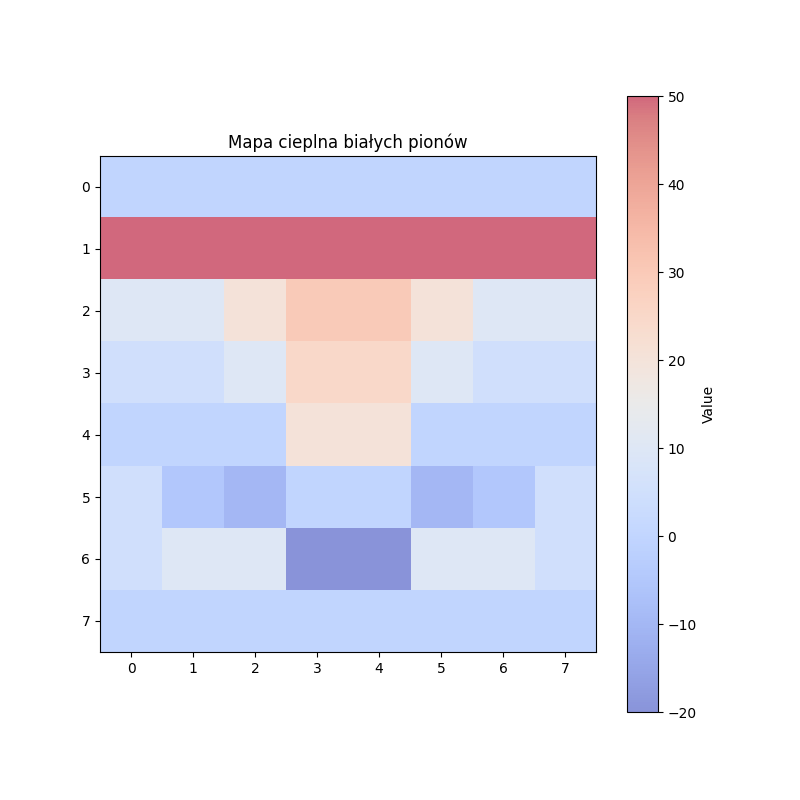
\includegraphics[width=0.5\textwidth]{rozdzialy/rozdzial02/2_ulepszenia_oceny/rysunki/bialePiony}
        &
        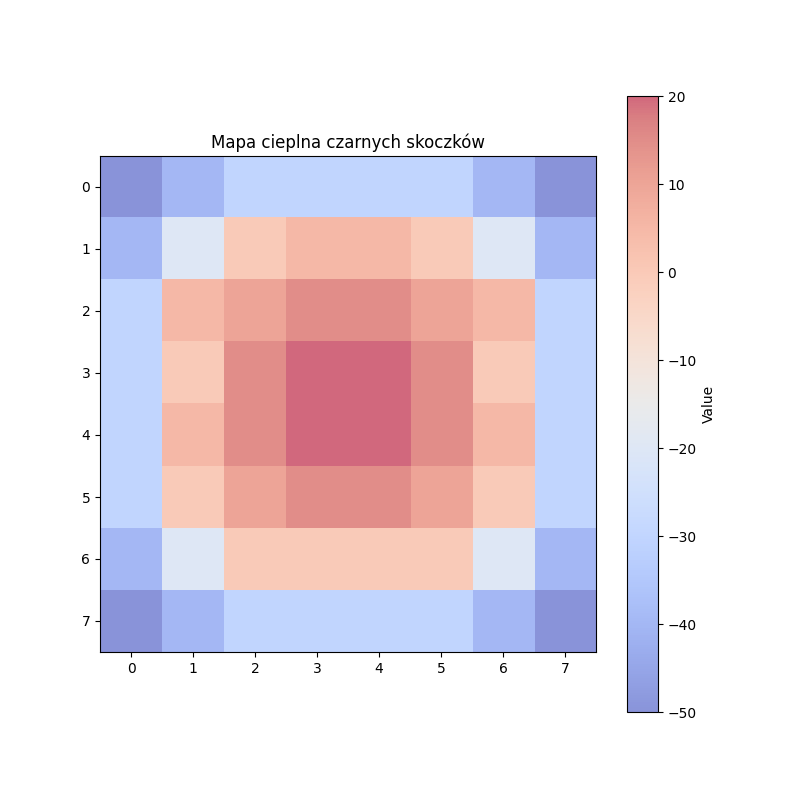
\includegraphics[width=0.5\textwidth]{rozdzialy/rozdzial02/2_ulepszenia_oceny/rysunki/czarneSkoczki}
    \end{tabular}
    \caption{Przykładowe tablice cieplne bierek: a) białych pionów, b) czarnych skoczków}
    \label{fig: tablice-figur}
\end{figure}

Rezultatem zastosowania tablic figur stał się silnik, który w odczuciu autora znacznie lepiej \enquote{rozumiał} pozycję na planszy.
\subsection{Ochrona króla}
\label{subsec:ochrona-krola}

{
    \color{red}
    \large Sprawdzanie, czy król jest chroniony, na przykład przez piony
}
\subsection{Struktura pionów}
\label{subsec:struktura-pionow}

\subsubsection{Opis zagadnienia}
Po implementacji ulepszenia \ref{subsec:tablice-figur} silnik zyskał zdolność oceny pozycyjnej.
Niedoskonałością było natomiast, że bierki oceniane były pojedynczo, to jest bez uwzględnienia ich wzajemnych relacji, oraz relacji w stosunku do bierek przeciwnika.
Było to szczególnie przydatne w przypadku pionków.
Termin \enquote{struktura pionów} jest szeroko znany w literaturze szachowej \cite*{stuktura-pionow} i odnosi się do technik mających na celu skoordynowaną obronę własnej części szachownicy oraz przeprowadzania ataków z wykorzystaniem pionów.
Skuteczne pozycjonowanie pionków na planszy może prowadzić do uzyskania przewagi w grze.

\subsubsection{Implementacja}
Zasady rozumiane przez graczy szachowych w sposób intuicyjny należało przekształcić na zbór reguł możliwych do zrozumienia przez program, a prowadzących do skutecznej oceny pozycji.
\begin{itemize}
    \item Pionki, które posiadają z tyłu po swojej prawej lub lewej stronie innego pionka, są uważane za dobrze chronione.
    \item Pionki nieposiadające za sobą innych pionków na sąsiednich kolumnach są traktowane jako izolowane i trudne do obrony.
    \item Dwa pionki znajdujące się w jednej linii pionowej (tzw. \enquote{zdublowane}) są uważane za~małowartościowe, gdyż odsłaniają inne linie na potencjalne ataki.
    \item Pionki, dla których istnieje możliwość promocji, spowodowana brakiem pionów przeciwnika na sąsiednich kolumnach, są uznawane za bardzo wartościowe.
\end{itemize}

Powyższe techniki zostały w dużej mierze zaimplementowane z wykorzystaniem uprzednio zainicjowanych tablic bitowych bierek i operacjach na nich.
Odbyło się to w sposób analogiczny do generowania dostępnych ruchów.

\subsubsection{Rezultat}
Rezultatem stał się silnik, który w sposób bardziej złożony oraz koherentny był w stanie ocenić swoją sytuację na planszy.
Istniało natomiast ryzyko, że czas konieczny na przeprowadzanie koniecznych obliczeń znacząco przewyższy oferowane korzyści.
Nie sposób było to sprawdzić w trakcie zwykłej gry przeciw silnikowi.
Rzeczywiste efekty przedstawiono w rozdziale \ref{ch: ocena-sily-silnika}.
%\subsection{Moment gry \colorbox{red}{TODO}}
\label{subsec:moment-gry}

{
    \color{red}
    \large Początek - środek - koniec.
    Różne wartości, szczególnie dla króla w zależności od momentu gry.
}
\subsection{Mobilność}
\label{subsec:mobilnosc}
\textit{Usprawnia pozycjonowanie hetmana, wieży i gońca.}


\subsubsection{Opis zagadnienia}
\subsubsection{Implementacja}
\subsubsection{Rezultat}
%\subsection{Algorytm genetyczny}
\label{subsec:genetyczny}
\begin{center}
    \textcolor{red}{\textbf{BEZ IMPLEMENTACJI, SAM OPIS}}
\end{center}

\subsubsection{Opis zagadnienia}



